\documentclass{article}

\usepackage[most]{tcolorbox}
\usepackage{physics}
\usepackage{graphicx}
\usepackage{float}
\usepackage{amsmath}
\usepackage{amssymb}


\usepackage[utf8]{inputenc}
\usepackage[a4paper, margin=1in]{geometry} % Controla los márgenes
\usepackage{titling}

\title{Clase 25 }
\author{Manuel Garcia.}
\date{\today}

\renewcommand{\maketitlehooka}{%
  \centering
  \vspace*{0.05cm} % Espacio vertical antes del título
}

\renewcommand{\maketitlehookd}{%
  \vspace*{2cm} % Espacio vertical después de la fecha
}

\newcommand{\caja}[3]{%
  \begin{tcolorbox}[colback=#1!5!white,colframe=#1!25!black,title=#2]
    #3
  \end{tcolorbox}%
}

\begin{document}
\maketitle

\section{Haces tangentes }
Un haz tangente a una variedad $ M  $ es el conjunto de todos los espacios tangentes de esta variedad: 
\begin{gather*}
  TM = \underset{p\in M }{\cup}T_p M  \qquad M \text{ es el espacio base de }TM. \quad \forall p \in M 
\end{gather*}
Podemos elegir $ (x ^ {i }(p) , \xi ^ {i }(p) ) \in TM$. En el espacio tangente tenemos unos elementos $ u ^ {\alpha}(p) = (x ^ {i }(p), \xi ^ {i }(p)) $ con $ \alpha = 1,...,2m  $. \textbf{Localmente} lo podemos escribir como (esto lo podemos ver como un espacio de fase): 
\begin{gather*}
  TM = u_i \times T_pM = u_i \times \mathbb{R}^ {m } 
\end{gather*}

\textbf{EJEMPLOS}

\textbf{Proyección }
\begin{gather*}
  \pi : TU _{i } \rightarrow U _{i } ,\quad \forall u \in T U_i \\
  \pi(u) = p \in U_i \\
  \pi ^ {-1 }(p) = T_p M \rightarrow \text{ Fibra en }p .
\end{gather*}
\begin{figure}[H]
  \begin{center}
    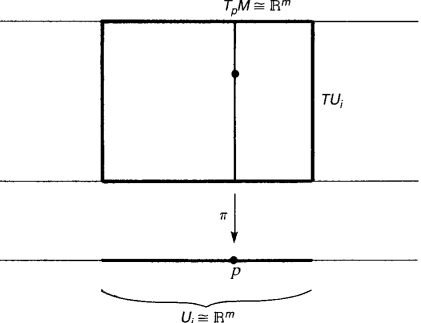
\includegraphics[width=0.4\textwidth]{proyeccion.png}
  \end{center}
\end{figure}
\textbf{Cambios de coordenadas }
\begin{gather*}
  (U_i,x ^ {\mu }), (U_j,y ^ {\mu }), \quad y ^ {\mu }= \psi(p) \\
  V ^ {'\mu }(y) = \frac{\partial y ^ {\mu } }{\partial x ^ {\nu }}V ^ {\nu }(x) = J _{\nu } ^ {\mu } V ^ {\nu }(x) \\
  J _{\nu } ^ {\mu } \in GL(n, \mathbb{R}^ {n }) \rightarrow \text{ Grupo de estructura de }TM. 
\end{gather*}
El mapeo $ s\ : \ M \rightarrow TM/ \ \pi \circ s = id_M \text{ Es una sección. } $\\
El mapeo $ x_i : U_i \rightarrow TU_i / \ \pi \circ s_i = is_M $ es una sección local.

\hfill

\hfill 

\hfill 

Haciendo uso del espacio tangencial podemos definir unas fibras a lo largo del espacio. 

\section{Haces Fibrados }
Un haz fibrado diferenciable $ (E,\pi,M,F,G) $ se compone de los siguientes elementos: 
\begin{itemize}
  \item Una variedad diferenciable $ E \rightarrow  $ espacio total. 
  \item Una variedad diferenciable $ M \rightarrow  $ espacio base. 
  \item Una variedad diferenciable $ F \rightarrow  $ fibra (o fibra típica). 
  \item Una función surjectiva $ \pi: E \rightarrow M \rightarrow \text{proyección, }\pi ^ {-1 }(p) = F _{p } \approx F  $ fibra en $ p  $.
  \item Un grupo de Lie $ G  $ con acción sobre $ F  $ a la izquierda $ \quad \rightarrow \quad  $ grupo de estructura. 
  \item Una cubertura de $M, \{ U_i \}$ con un difeomorfismo. 
    \begin{gather*}
      \phi_i : U_i \times F \rightarrow \pi ^ {-1 }(U_i) / \pi\circ \phi_i (p,f) = p \rightarrow \text{trivialización local.}\\
      \phi _{i }  ^ {-1 }: \pi ^ {-1 }(U_i ) \rightarrow U_i \times F 
    \end{gather*}
  \item $ \phi_i (p,f) = \phi _{i,p } (f), \quad \phi _{j,p } : F \rightarrow F  $ sea un elemento de $ G  $. Las funciones $ \phi_i,\phi_j  $ se relacionan por un mapeo suave $ t _{ij } : U_i \cap U_j \rightarrow G / \quad \phi_j (p,f) = \phi_i (p,t _{ij } (p)f ) $. $ t _{ij } \rightarrow  $ funciones de transición.
\end{itemize}

\subsection{Haces Vectoriales } 
Un haz vectorial tiene como fibra $ F  $ un espacio vectorial $ E \overset{\pi}{\rightarrow } M $. La fibra $ F  $ tiene dimensión $ k  $ la cual se denomina dimensión de la fibra. Las funciones de transición en la fibra $ \in GL(k, \mathbb{R}) $. 

\subsection{Haces principales }
Un haz principal tiene fibra $ F  $ la cual es identica al gurpo de estructura $ G  $. $ P \overset{\pi}{\rightarrow }M \circ P(M,G) $ también se llama un haz $ G  $ sobre $ M  $.

\subsection{Haces cotangentes }
\begin{gather*}
  T^* M \equiv \underset{p \in M }{\cup }T^*_p M 
\end{gather*}


\end{document}
